% Created 2023-10-01 Sun 16:40
% Intended LaTeX compiler: pdflatex
\documentclass[12pt, a4paper]{article}
\usepackage[utf8]{inputenc}
\usepackage[T1]{fontenc}
\usepackage{graphicx}
\usepackage{longtable}
\usepackage{wrapfig}
\usepackage{rotating}
\usepackage[normalem]{ulem}
\usepackage{amsmath}
\usepackage{amssymb}
\usepackage{capt-of}
\usepackage{hyperref}
\usepackage{placeins}
\usepackage{gensymb}
\usepackage[letterpaper]{geometry}
\geometry{top=1.0in, bottom=1.0in, left=1.0in, right=1.0in}
\usepackage{rotating}
\usepackage{graphicx}
\usepackage{pgfplots}
\usepackage{filecontents}
\usepackage{tikz}
\usepackage{fancyhdr}
\usepackage{enumitem}
\pagestyle{fancy}
\lhead{}
\chead{}
\rhead{Johnson \thepage}
\lfoot{}
\cfoot{}
\rfoot{}
\renewcommand{\headrulewidth}{0pt}
\renewcommand{\footrulewidth}{0pt}
\setlength\headsep{0.333in}
\newcommand{\bibent}{\noindent \hangindent 40pt}
\newenvironment{workscited}{\newpage \begin{center} Works Cited \end{center}}{\newpage }
\graphicspath{ {./attachments} }
\author{Christian}
\date{\today}
\title{}
\hypersetup{
 pdfauthor={Christian},
 pdftitle={},
 pdfkeywords={},
 pdfsubject={},
 pdfcreator={Emacs 28.2.50 (Org mode 9.7-pre)}, 
 pdflang={English}}
\begin{document}

\begin{document}
\begin{flushleft}
Christian Johnson\\
\vspace{2mm}Dr. Paul Crilly\\
\vspace{2mm}Antennas and Propogation\\
\vspace{2mm}September 27 2023\\
\vspace{4mm}\begin{center}
Lab 3 Report
\end{center}
\vspace{1mm}\setlength{\parindent}{0.5in}

\begin{Abstract}
In this laboratory exploration of transmission lines, standing waves, and their practical implications, we delved into the principles of SWR (Standing Wave Ratio) and the precision required for frequency measurement using a slotted line apparatus. Our practical experiments demonstrated the relationship between load conditions and SWR, emphasizing the significance of lead lengths. We observed that longer lead lengths correlate with higher SWR values, while shorter leads exhibit lower SWR. These findings underscore the practical importance of load conditions in transmission line behavior.

Furthermore, our investigation revealed that the frequency of the source significantly influences SWR values. Changes in source frequency alter the standing wave patterns and, consequently, the load impedance seen by the line, directly impacting SWR. Additionally, we examined the impact of frequency on resistive loads, noting that at higher frequencies, resistors with shorter lead lengths become increasingly reactive.

In summary, this laboratory exercise served as a platform for improving our comprehension of transmission lines, standing waves, and the practical applications of SWR. It allowed us to explore how load conditions, source frequency, and lead lengths interact, ultimately enriching our understanding of these fundamental concepts in electrical engineering.
\end{Abstract}
\section*{Procedures}
\label{sec:org734a263}
Our laboratory inquiry revolved around the dynamics of transmission lines and their interaction with standing waves. The primary objectives encompassed a fundamental grasp of SWR (Standing Wave Ratio) principles and the precision required to measure an unknown frequency. The following section details the procedures that guided our exploration.
For our experiments, we used several components: the slotted line, the 8648B waveform generator, and an oscilloscope. Initially, we delegated a classmate to set the waveform generators frequency - this was to ensure that the measurements we were taking were unbiased. 
As we moved the copper sensor probe along the slotted line, we observed a series of amplitude variations. Our experiment hinged on identifying and recording the valleys in our graph - points where the RMS voltage approaches a minima. We marked these points along the slotted line, recording the locations where the voltage minimums occured.
Our calculations yielded the frequency of the waveform generator, inferred from the measured slotted line wavelength.
After working on this experiment, we began to examine the impact of lead length on SWR. Using three different loads with varying lead lengths, we used the 9912A analyzer to measure SWR, determining where that value began to exceed 2.
\section*{Results}
\label{sec:org86e9aa5}

As we progressed though these processes, we recorded a wide variety of results. Our investigation commenced with the examination of SWR (Standing Wave Ratio) for various lead lengths, shedding light on the influence of load conditions. 
For the longest lead, we recorded SWR=2 at 141.4 MHz, with a Wavelength of 2.12 meters and Lead Length of 5 cm for a Length-to-Wavelength Ratio of 0.023 lambda. The middle lead yielded an SWR=2 observed at 368.03 MHz, Wavelength of 0.8151 meters, and Lead Length of 0.0125 meters for a Length-to-Wavelength Ratio of 0.015 lambda. Finally, the Ideal Load gave an SWR=2 observed at 3440.280 MHz. These measurements illustrate the varying SWR values at different lead lengths, offering insights into the relationship between lead length and SWR.
In the second part of our exploration, we focused on the slotted line, probing its behavior at distinct positions. At 0.7 M, we recorded a frequency of 450 MHz, 525 MHz at 0.573 M, and 310 MHz at 0.975 M. These measurements in the slotted line section allowed us to examine how signal frequencies varied with position along the slotted line, contributing to our understanding of standing wave patterns.
These findings form a vital part of our experiment, demonstrating the practical implications of transmission line behavior and standing waves under different load conditions. The exploration of SWR highlights the significance of load lengths, while the observations in the slotted line section shed light on frequency variations along the line.
\section*{Conclusions}
\label{sec:org5a3552a}
Over the course of our investigation into transmission lines, standing waves, and their practical applications, several key conclusions emerge.
Our examination of SWR at different lead lengths demonstrated a clear correlation between load length and SWR values. Specifically, longer lead lengths corresponded to lower SWR values, while shorter leads resulted in higher SWR. This underscores the importance of load conditions in transmission line behavior. In the slotted line section, we observed fluctuations in signal frequencies at distinct positions. This variation in frequency along the slotted line highlighted the presence of standing wave patterns and their impact on signal behavior. Our experiment demanded precision in measuring an unknown frequency. The calculated frequency, based on the measured slotted line wavelength, allowed for accurate comparison with the generator's readout. This process served as a testament to the rigor of our measurements.
In summation, our exploration unveiled the intricate relationship between load conditions and SWR, emphasized the significance of standing wave patterns in signal behavior, and showcased the precision achievable in frequency measurements. These findings not only enrich our understanding of transmission lines and standing waves but also underscore their practical importance in the field of electrical engineering.

\newpage
\begin{center}
Appendices
\end{center}

\begin{figure}[htb]
\centering
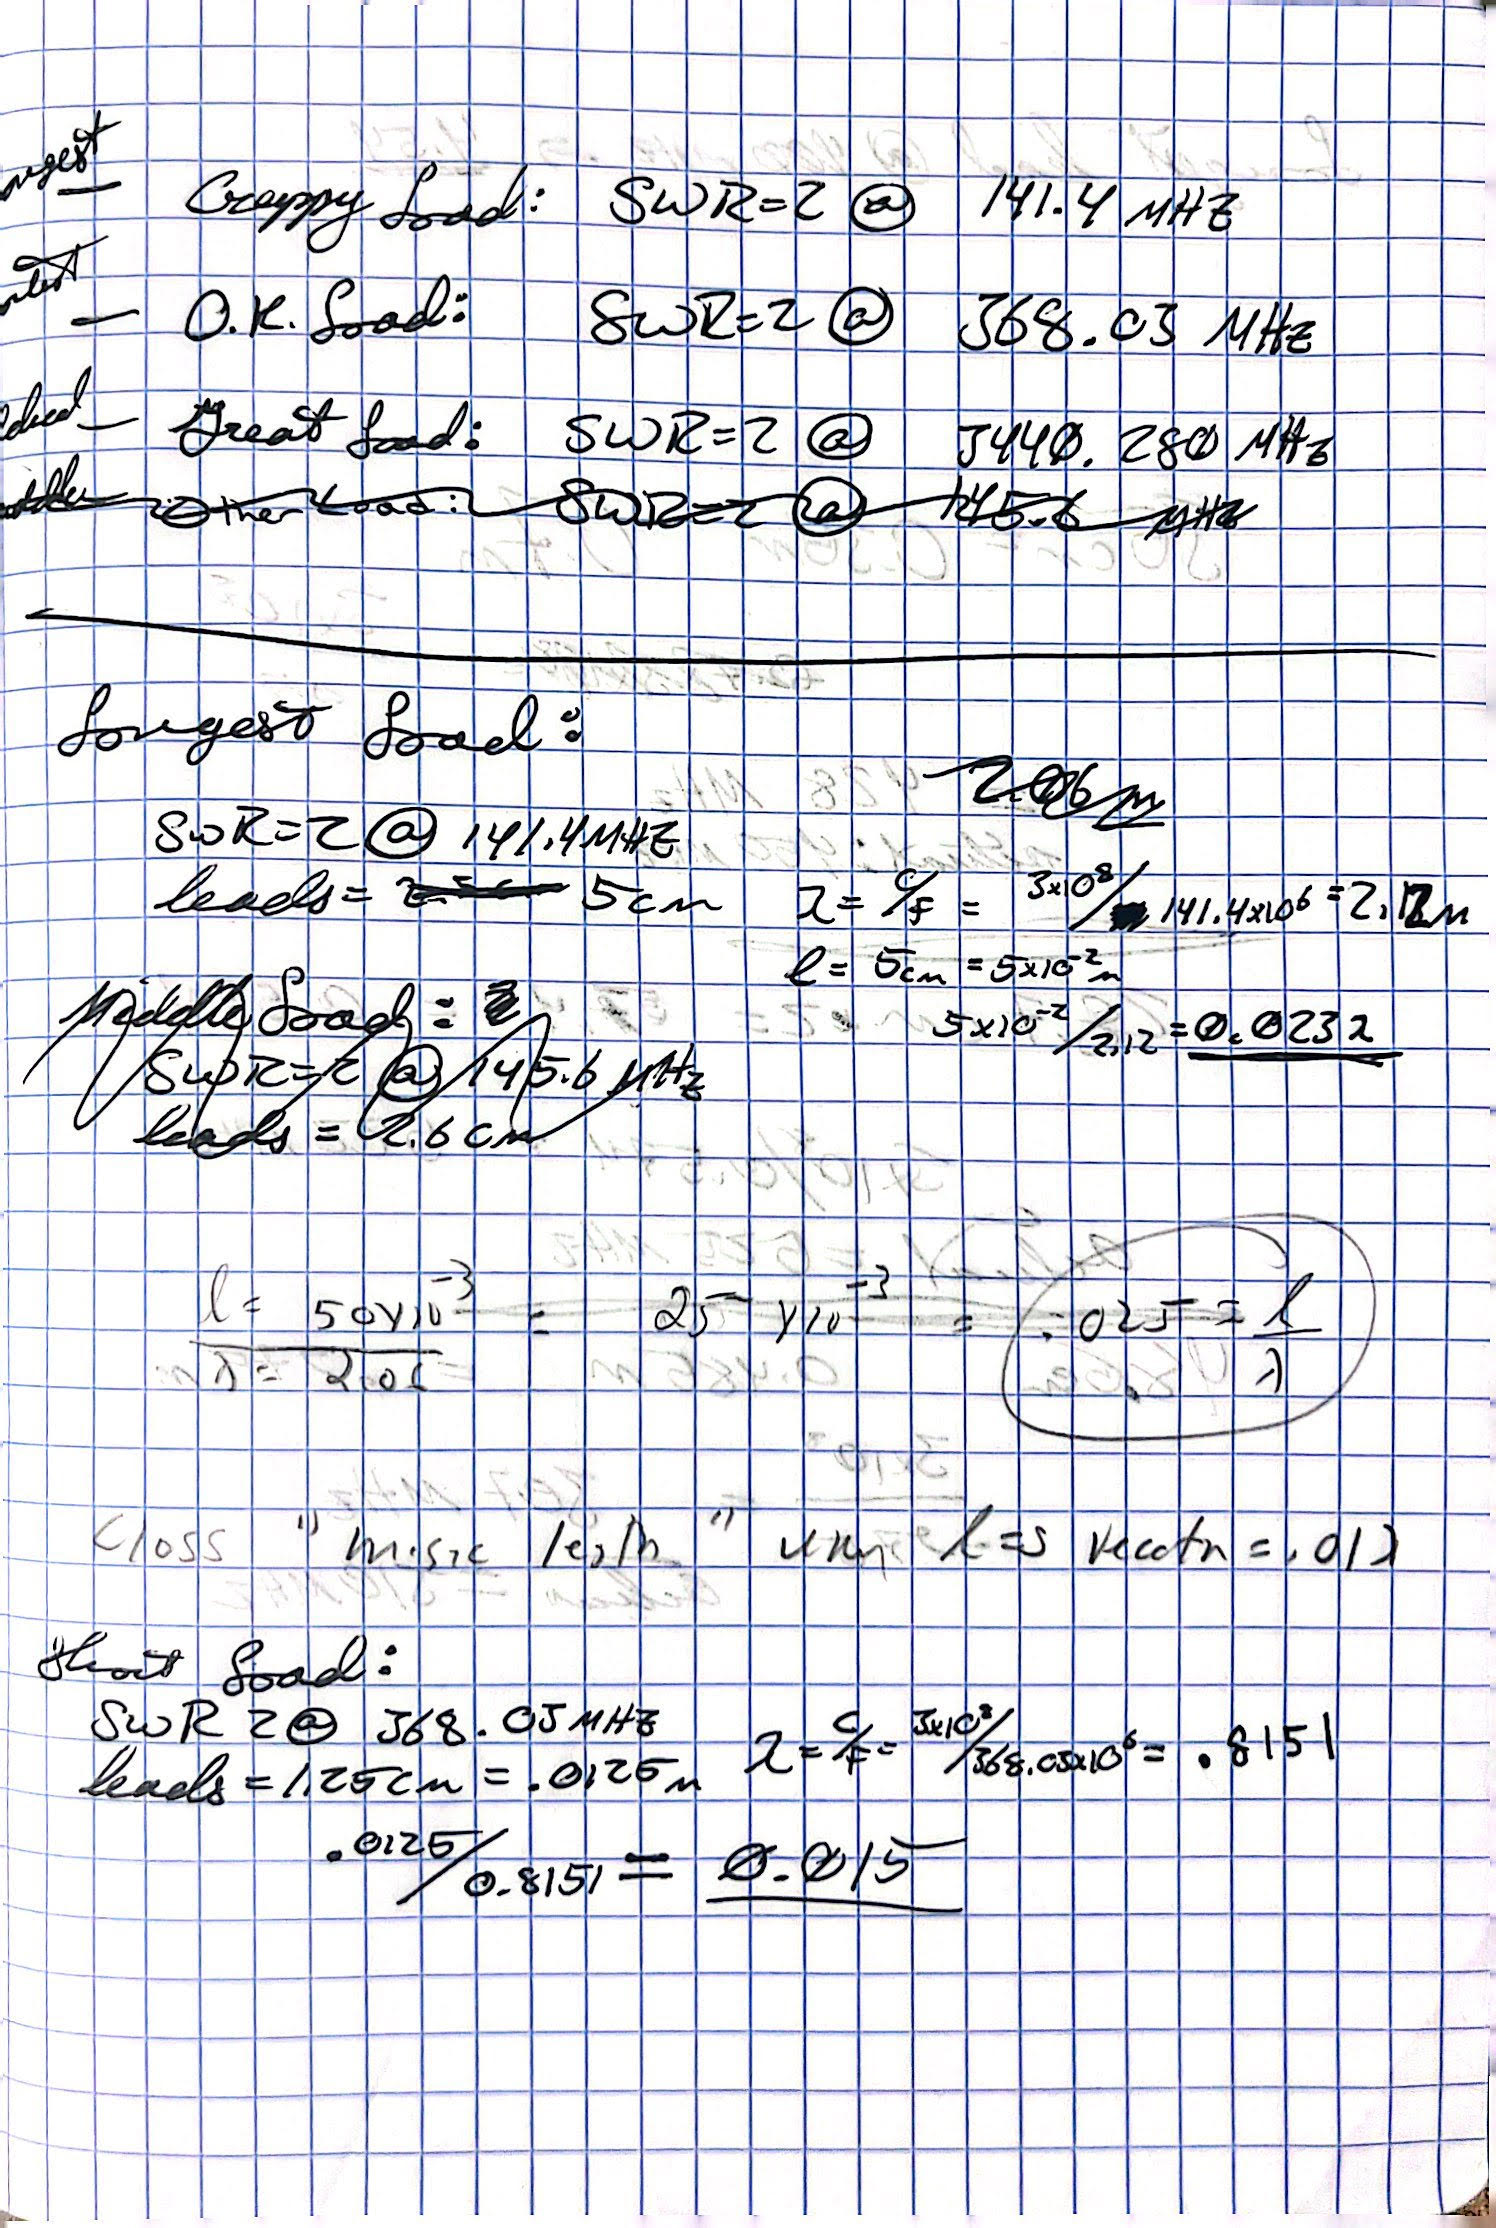
\includegraphics[width=0.5\textwidth]{LabNotebook1.jpg}
\caption{Notebook Page 1}
\end{figure}
\newpage
\begin{figure}[htb]
\centering
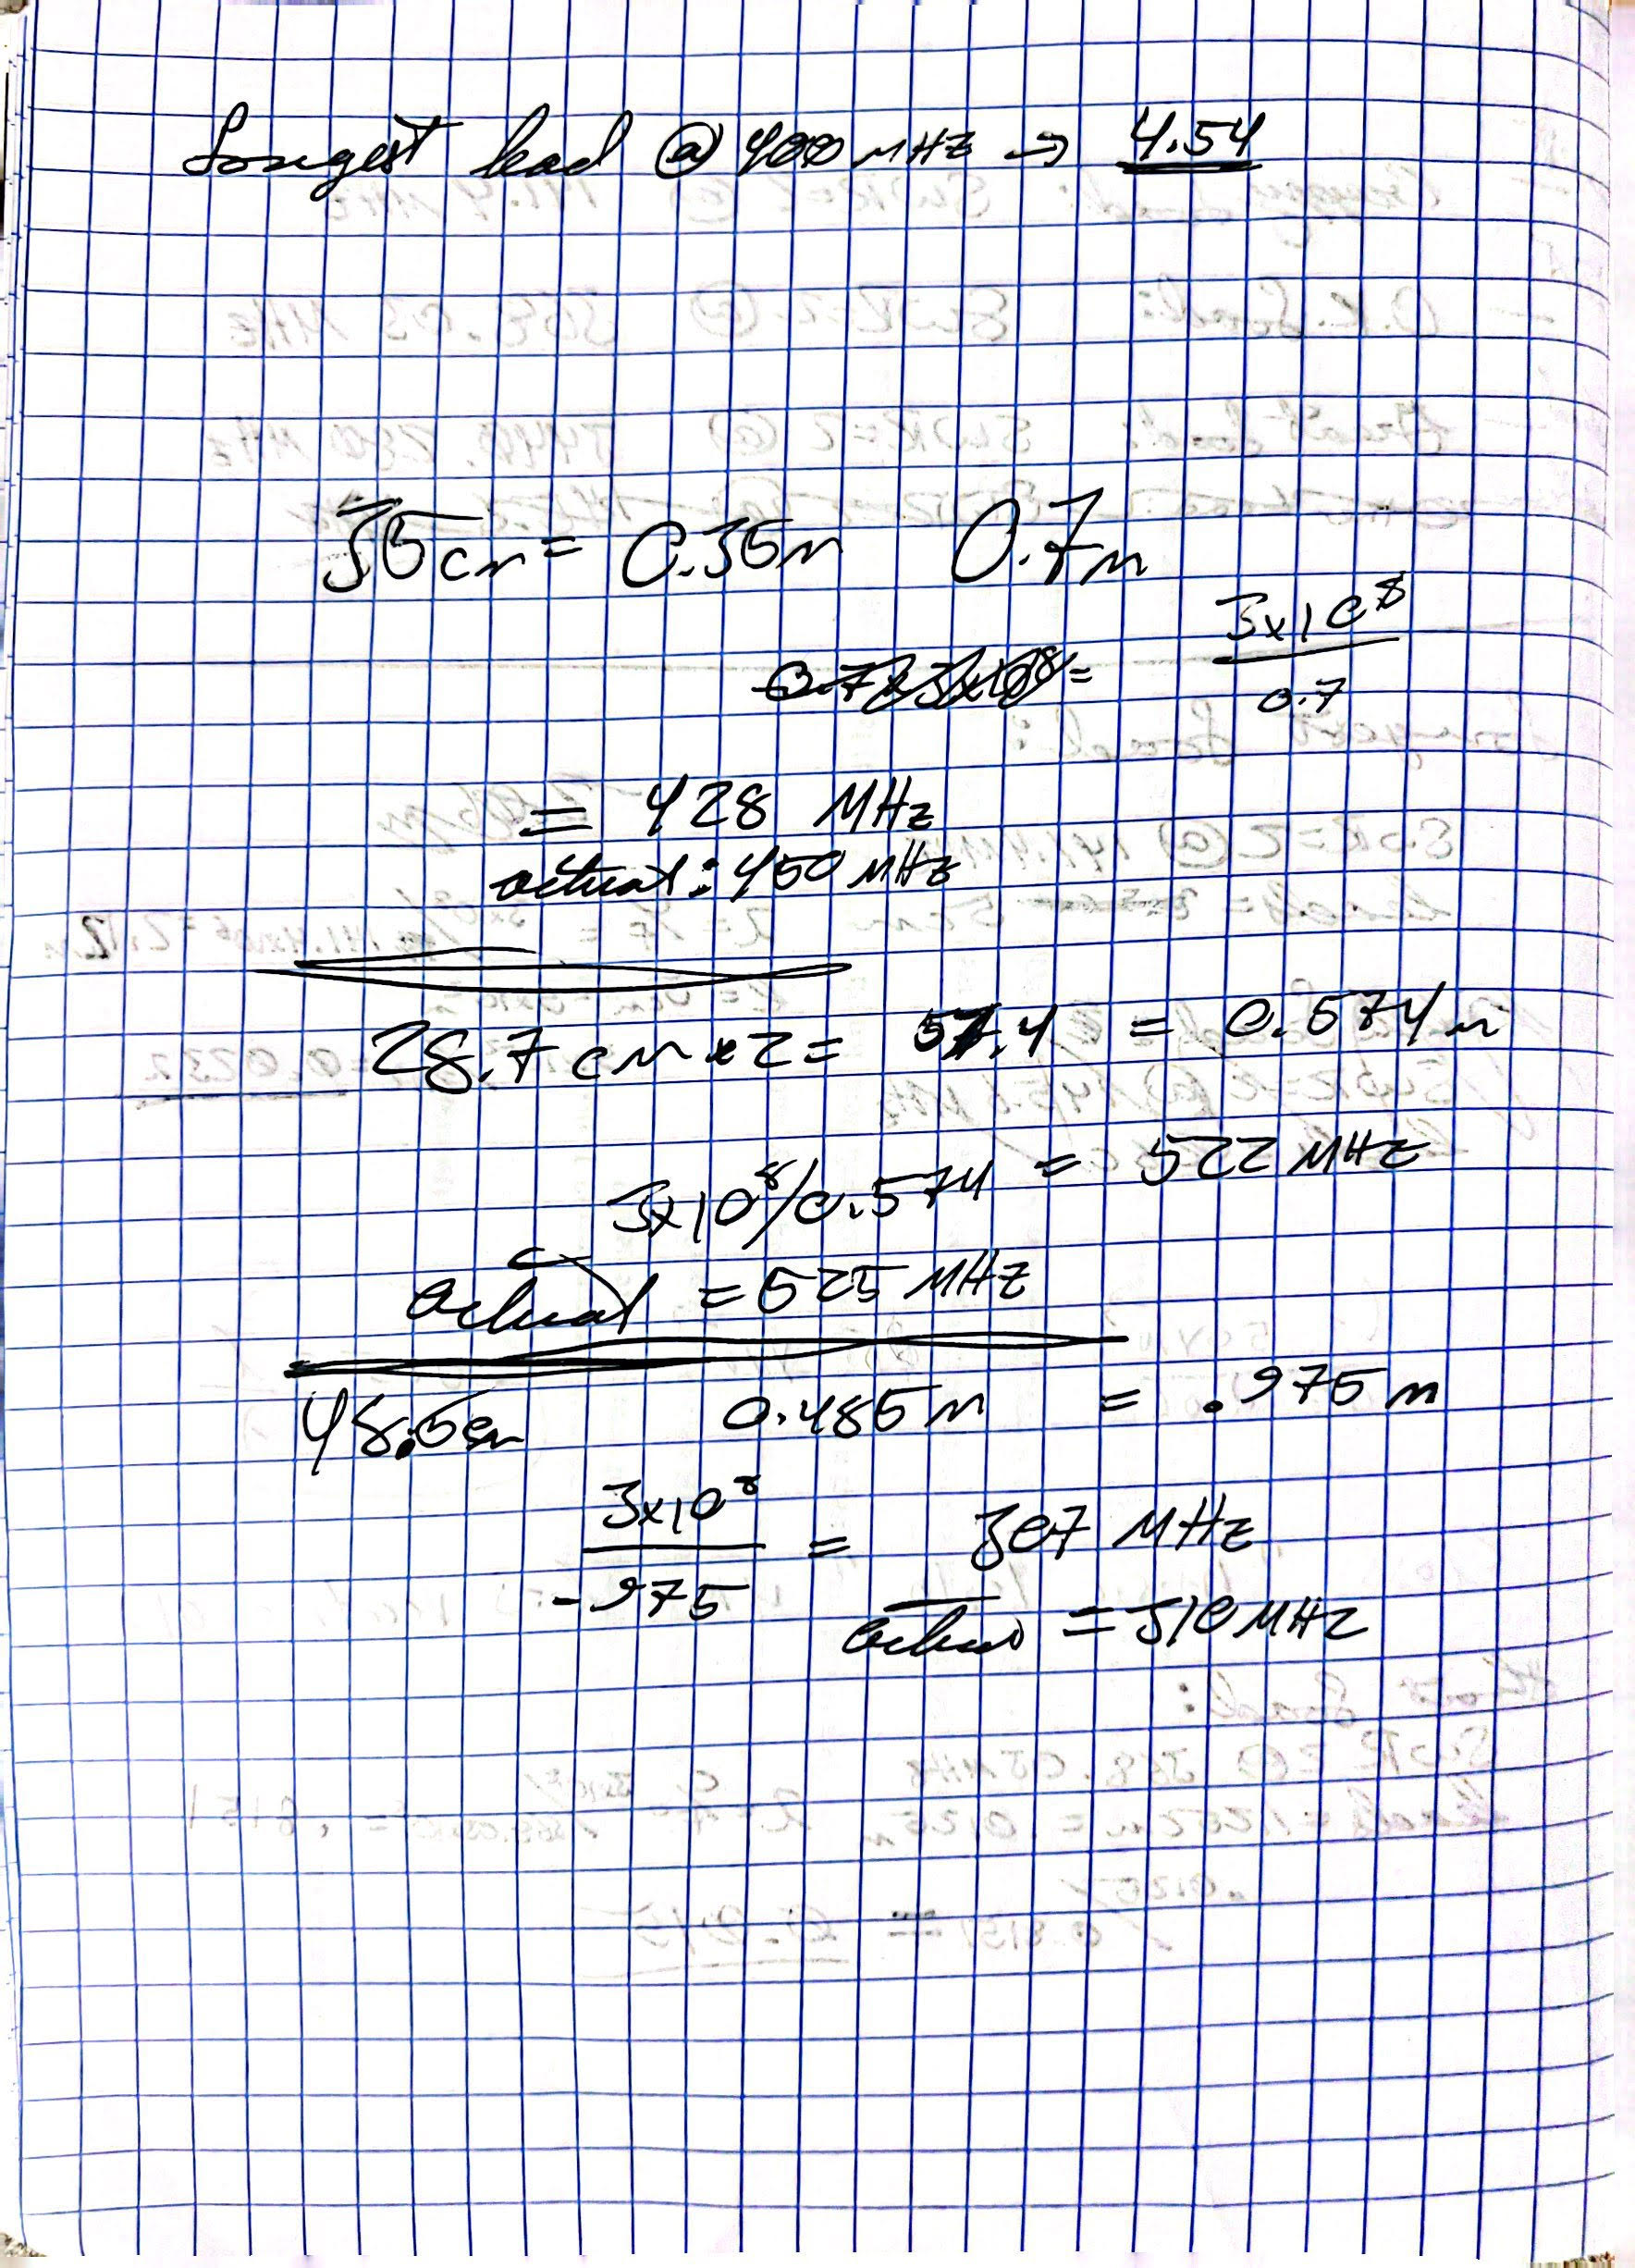
\includegraphics[width=0.5\textwidth]{LabNotebook2.jpg}
\caption{Notebook Page 2}
\end{figure}
\newpage

\begin{center}
Lab Questions
\end{center}
\vspace{2mm}
\begin{enumerate}[label=\textbf{\arabic*.}]
\item What affected the accuracy of the frequency measurement? What changes in the apparatus might increase the accuracy and precision of your measurement?
Several fators affected our accuracy, including variations in signal amplitude, human error identifying precise values, and the imprecise anture of the slotted line measurements. In order to improve some of these, we could take steps to improve consistancy when placing the probe, or take other measures to improve the precision with which we can record numbers.
\item Did the source frequency affect SWR?
Yes,m the source frequency affected SWR. SWR is a function of load impedance and characteristic impedance. Since changes in frequency can alter the load impedance, this will change SWR.
\item Which load was most effected by frequency?
The load with the longest lead was most affected by variations in frequency. Since longer lead lengths result in greater variations in load impedance, this will lead to more pronounced changes in SWR as frequencies vary.
\item At what frequency would you expect a resistor with half inch lead lengths to no longer be pure resistance?
We would begin to see reactive components to the resistance once length begins to exceed 0.1*wavelength. Given a length of 2.5cm = 0.025 m, we would see a wavelength of 0.0025 m. This would lead to a frequency of $\frac{3*10^{8}}{0.0025} = 120$ Mhz.
\item State any insights you have learned in relation to the above questions as well as other observations you might have made.
The interaction between lead length and signal frequency plays a large role in determining SWR. Longer leads contribute to increased SWR, while shorter leads tend to reduce it. Additionally, standing wave patterns are a manifestation of this interaction.
\item Why would some loads have a non-monotonic SWR profile.
Non-monotonic SWR profiles indicate SWR values that do not consistantly increase or decrease with changing frequency. This comes about when load impedance leads to complex standing wave patterns with multiple peaks and valleys (typically due to variance in frequency or reflected waves at different frequencies).
\item Why was an SWR of 2 chosen as the break point where a load has significant resistance?
An SWR of 2 was chosen because it corresponds to a reflection coefficient of about 1/3. At this point, we see a significant mismatch in impedance. This represents a practical threshold where a load exhibits significant reactance. 
\end{enumerate}

\end{document}
\end{document}